\chapter*{Introduction}

\addcontentsline{toc}{chapter}{Introduction}


L'objectif de ce dossier est de vous expliquer de A à Z la mise en place d'un système avec capteurs permettant l'affichage en temps réel de différentes données comme la température, l'humidité ou encore la luminosité d'une pièce, d'un couloir, etc....

En premier lieu, nous allons nous attarder sur la partie matériel : \textit{La Raspberry Pi} (je vous laisserais le choix du genre, c'est une question qui divise la France comme bien d'autre)

\begin{figure}[H]
\begin{center}
	\makebox[\textwidth]{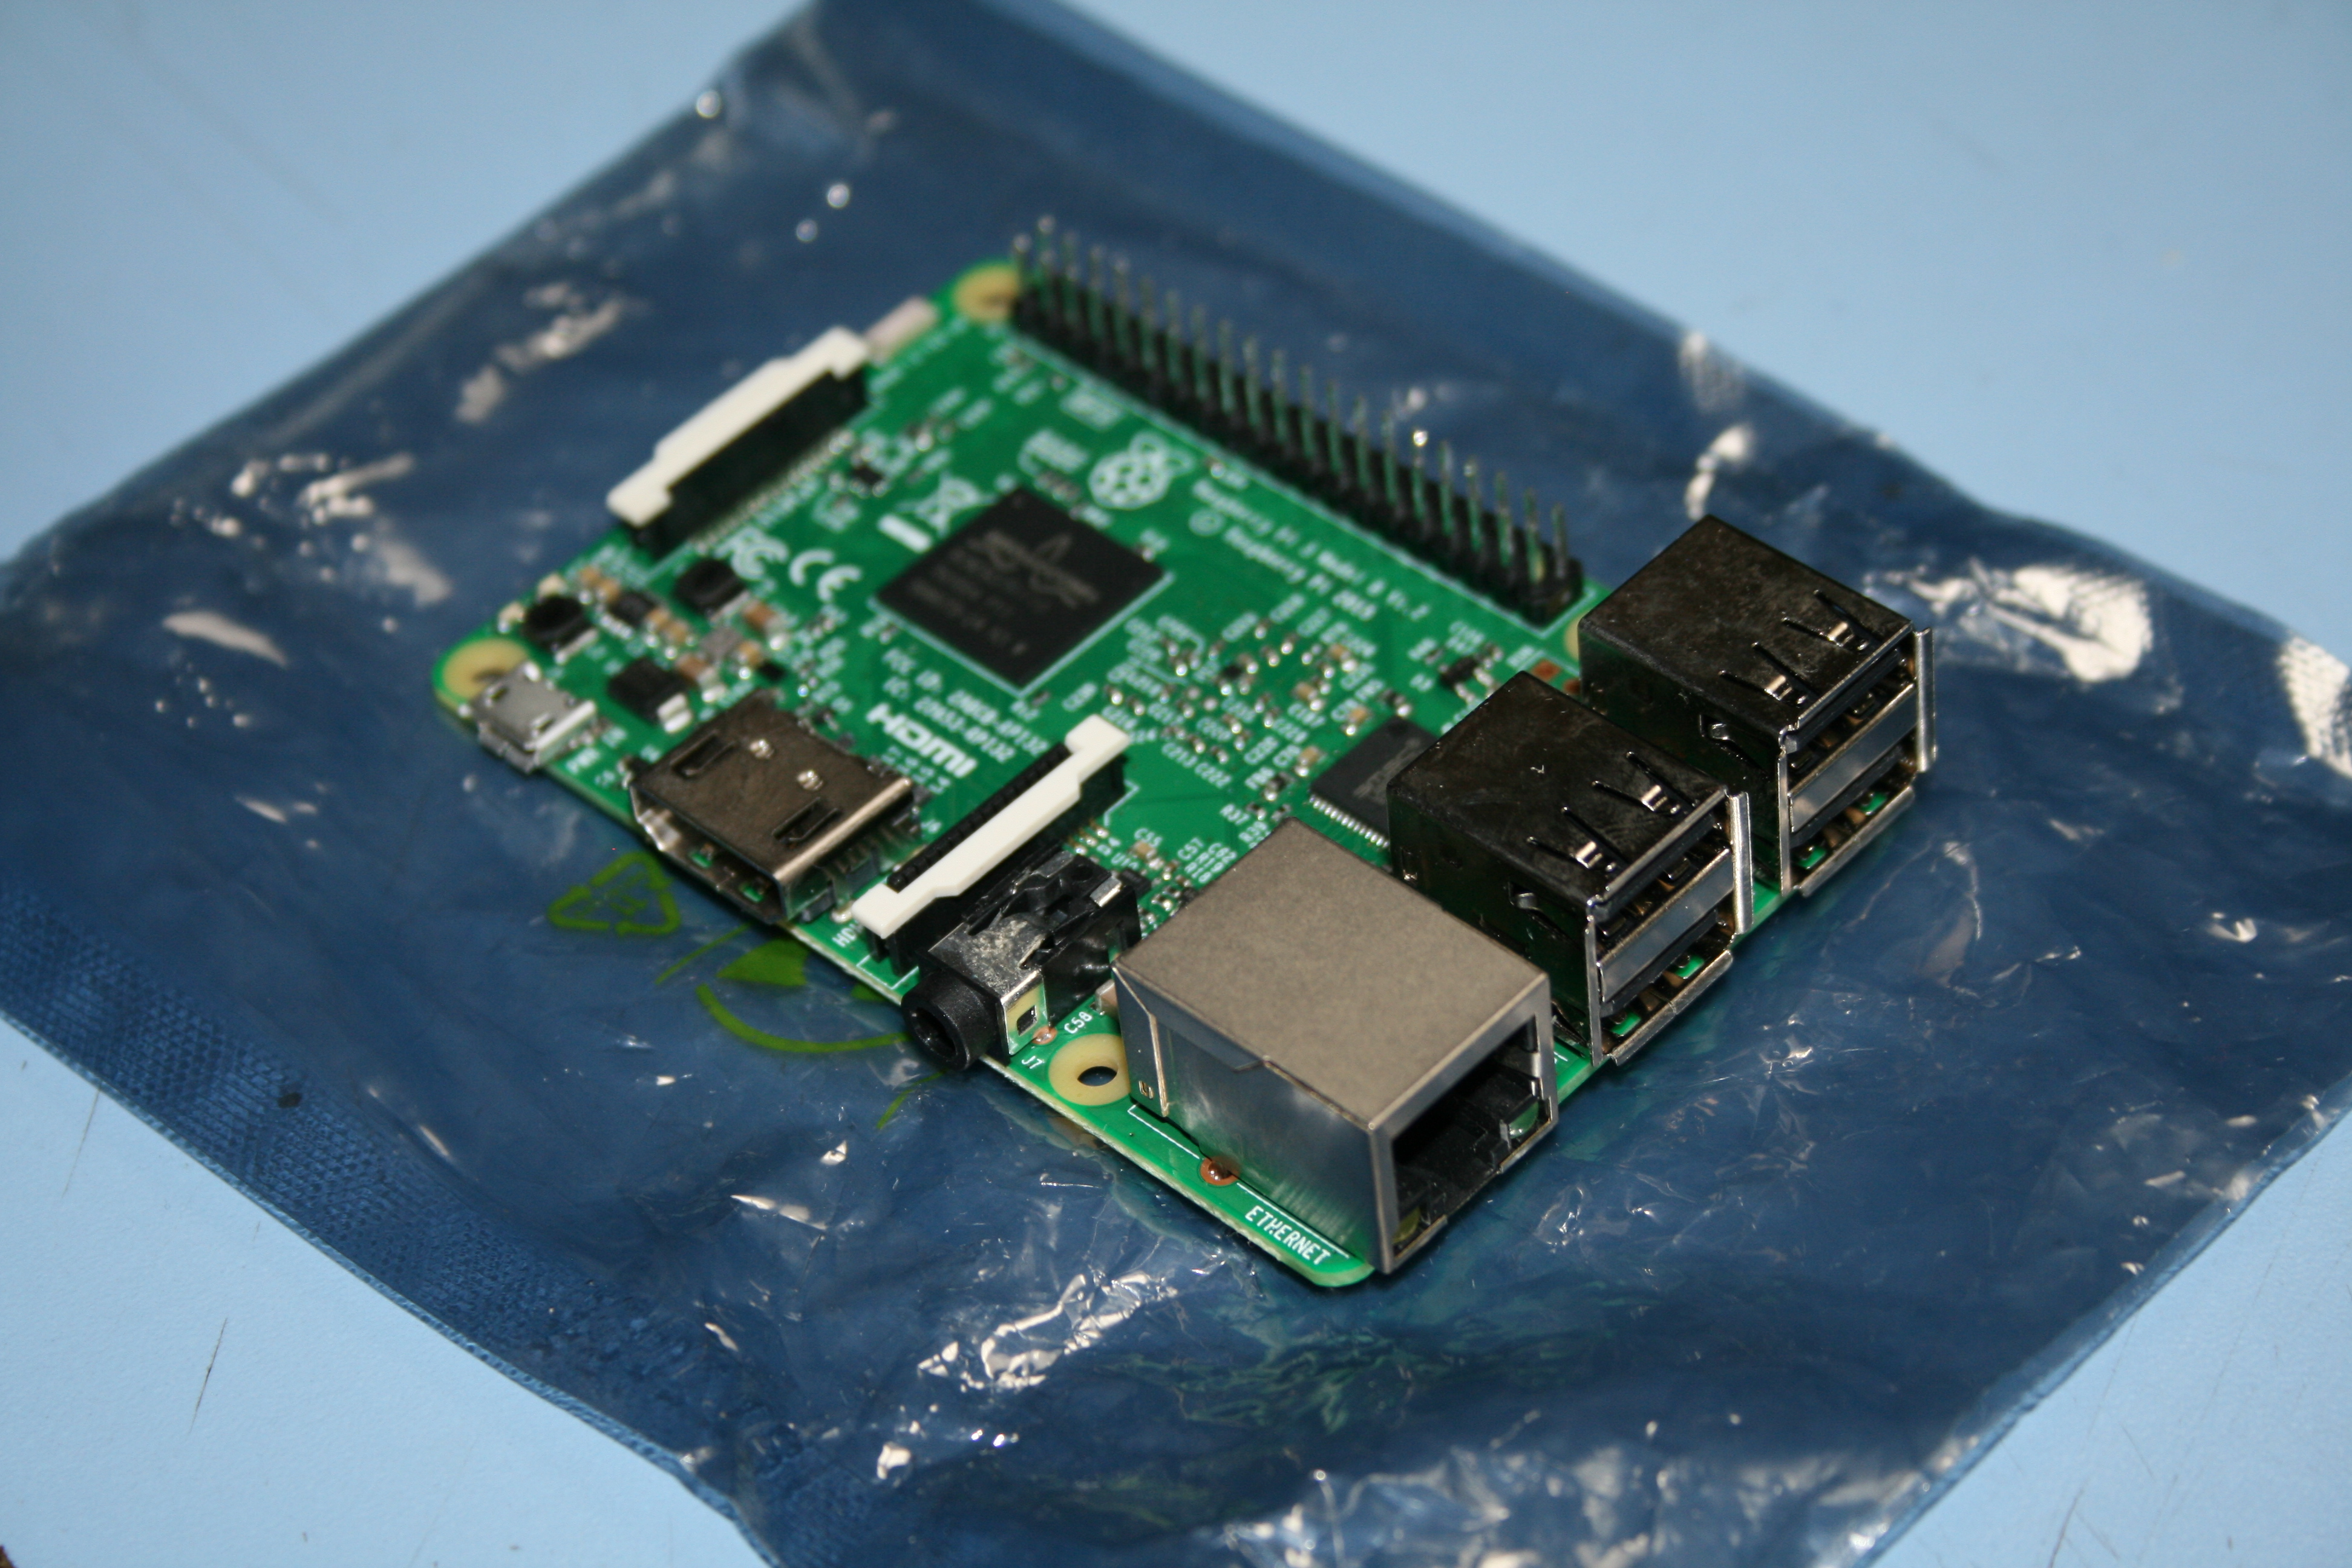
\includegraphics[width=.8\paperwidth]{images/rpi.jpg}}
\end{center}
	\caption{ \textit{Une RaspberryPi à nue}}
\end{figure}

Nous aborderons l'installation de capteur sur cette carte puis nous verrons l'installation logiciel.

Dans un second temps, nous verrons ensemble comment envoyer ces données dans le \textit{Cloud} mis en place par \textbf{Microsoft} : \textit{Azure} 

A la fin de ce dossier, vous serez en mesure de regarder n'importe où dans le monde la température ambiante de votre installation mais cessons de tergiverser et mettons nous au travail !